\documentclass[1p]{elsarticle_modified}
%\bibliographystyle{elsarticle-num}

%\usepackage[colorlinks]{hyperref}
%\usepackage{abbrmath_seonhwa} %\Abb, \Ascr, \Acal ,\Abf, \Afrak
\usepackage{amsfonts}
\usepackage{amssymb}
\usepackage{amsmath}
\usepackage{amsthm}
\usepackage{scalefnt}
\usepackage{amsbsy}
\usepackage{kotex}
\usepackage{caption}
\usepackage{subfig}
\usepackage{color}
\usepackage{graphicx}
\usepackage{xcolor} %% white, black, red, green, blue, cyan, magenta, yellow
\usepackage{float}
\usepackage{setspace}
\usepackage{hyperref}

\usepackage{tikz}
\usetikzlibrary{arrows}

\usepackage{multirow}
\usepackage{array} % fixed length table
\usepackage{hhline}

%%%%%%%%%%%%%%%%%%%%%
\makeatletter
\renewcommand*\env@matrix[1][\arraystretch]{%
	\edef\arraystretch{#1}%
	\hskip -\arraycolsep
	\let\@ifnextchar\new@ifnextchar
	\array{*\c@MaxMatrixCols c}}
\makeatother %https://tex.stackexchange.com/questions/14071/how-can-i-increase-the-line-spacing-in-a-matrix
%%%%%%%%%%%%%%%

\usepackage[normalem]{ulem}

\newcommand{\msout}[1]{\ifmmode\text{\sout{\ensuremath{#1}}}\else\sout{#1}\fi}
%SOURCE: \msout is \stkout macro in https://tex.stackexchange.com/questions/20609/strikeout-in-math-mode

\newcommand{\cancel}[1]{
	\ifmmode
	{\color{red}\msout{#1}}
	\else
	{\color{red}\sout{#1}}
	\fi
}

\newcommand{\add}[1]{
	{\color{blue}\uwave{#1}}
}

\newcommand{\replace}[2]{
	\ifmmode
	{\color{red}\msout{#1}}{\color{blue}\uwave{#2}}
	\else
	{\color{red}\sout{#1}}{\color{blue}\uwave{#2}}
	\fi
}

\newcommand{\Sol}{\mathcal{S}} %segment
\newcommand{\D}{D} %diagram
\newcommand{\A}{\mathcal{A}} %arc


%%%%%%%%%%%%%%%%%%%%%%%%%%%%%5 test

\def\sl{\operatorname{\textup{SL}}(2,\Cbb)}
\def\psl{\operatorname{\textup{PSL}}(2,\Cbb)}
\def\quan{\mkern 1mu \triangleright \mkern 1mu}

\theoremstyle{definition}
\newtheorem{thm}{Theorem}[section]
\newtheorem{prop}[thm]{Proposition}
\newtheorem{lem}[thm]{Lemma}
\newtheorem{ques}[thm]{Question}
\newtheorem{cor}[thm]{Corollary}
\newtheorem{defn}[thm]{Definition}
\newtheorem{exam}[thm]{Example}
\newtheorem{rmk}[thm]{Remark}
\newtheorem{alg}[thm]{Algorithm}

\newcommand{\I}{\sqrt{-1}}
\begin{document}

%\begin{frontmatter}
%
%\title{Boundary parabolic representations of knots up to 8 crossings}
%
%%% Group authors per affiliation:
%\author{Yunhi Cho} 
%\address{Department of Mathematics, University of Seoul, Seoul, Korea}
%\ead{yhcho@uos.ac.kr}
%
%
%\author{Seonhwa Kim} %\fnref{s_kim}}
%\address{Center for Geometry and Physics, Institute for Basic Science, Pohang, 37673, Korea}
%\ead{ryeona17@ibs.re.kr}
%
%\author{Hyuk Kim}
%\address{Department of Mathematical Sciences, Seoul National University, Seoul 08826, Korea}
%\ead{hyukkim@snu.ac.kr}
%
%\author{Seokbeom Yoon}
%\address{Department of Mathematical Sciences, Seoul National University, Seoul, 08826,  Korea}
%\ead{sbyoon15@snu.ac.kr}
%
%\begin{abstract}
%We find all boundary parabolic representation of knots up to 8 crossings.
%
%\end{abstract}
%\begin{keyword}
%    \MSC[2010] 57M25 
%\end{keyword}
%
%\end{frontmatter}

%\linenumbers
%\tableofcontents
%
\newcommand\colored[1]{\textcolor{white}{\rule[-0.35ex]{0.8em}{1.4ex}}\kern-0.8em\color{red} #1}%
%\newcommand\colored[1]{\textcolor{white}{ #1}\kern-2.17ex	\textcolor{white}{ #1}\kern-1.81ex	\textcolor{white}{ #1}\kern-2.15ex\color{red}#1	}

{\Large $\underline{12a_{1095}~(K12a_{1095})}$}

\setlength{\tabcolsep}{10pt}
\renewcommand{\arraystretch}{1.6}
\vspace{1cm}\begin{tabular}{m{100pt}>{\centering\arraybackslash}m{274pt}}
\multirow{5}{120pt}{
	\centering
	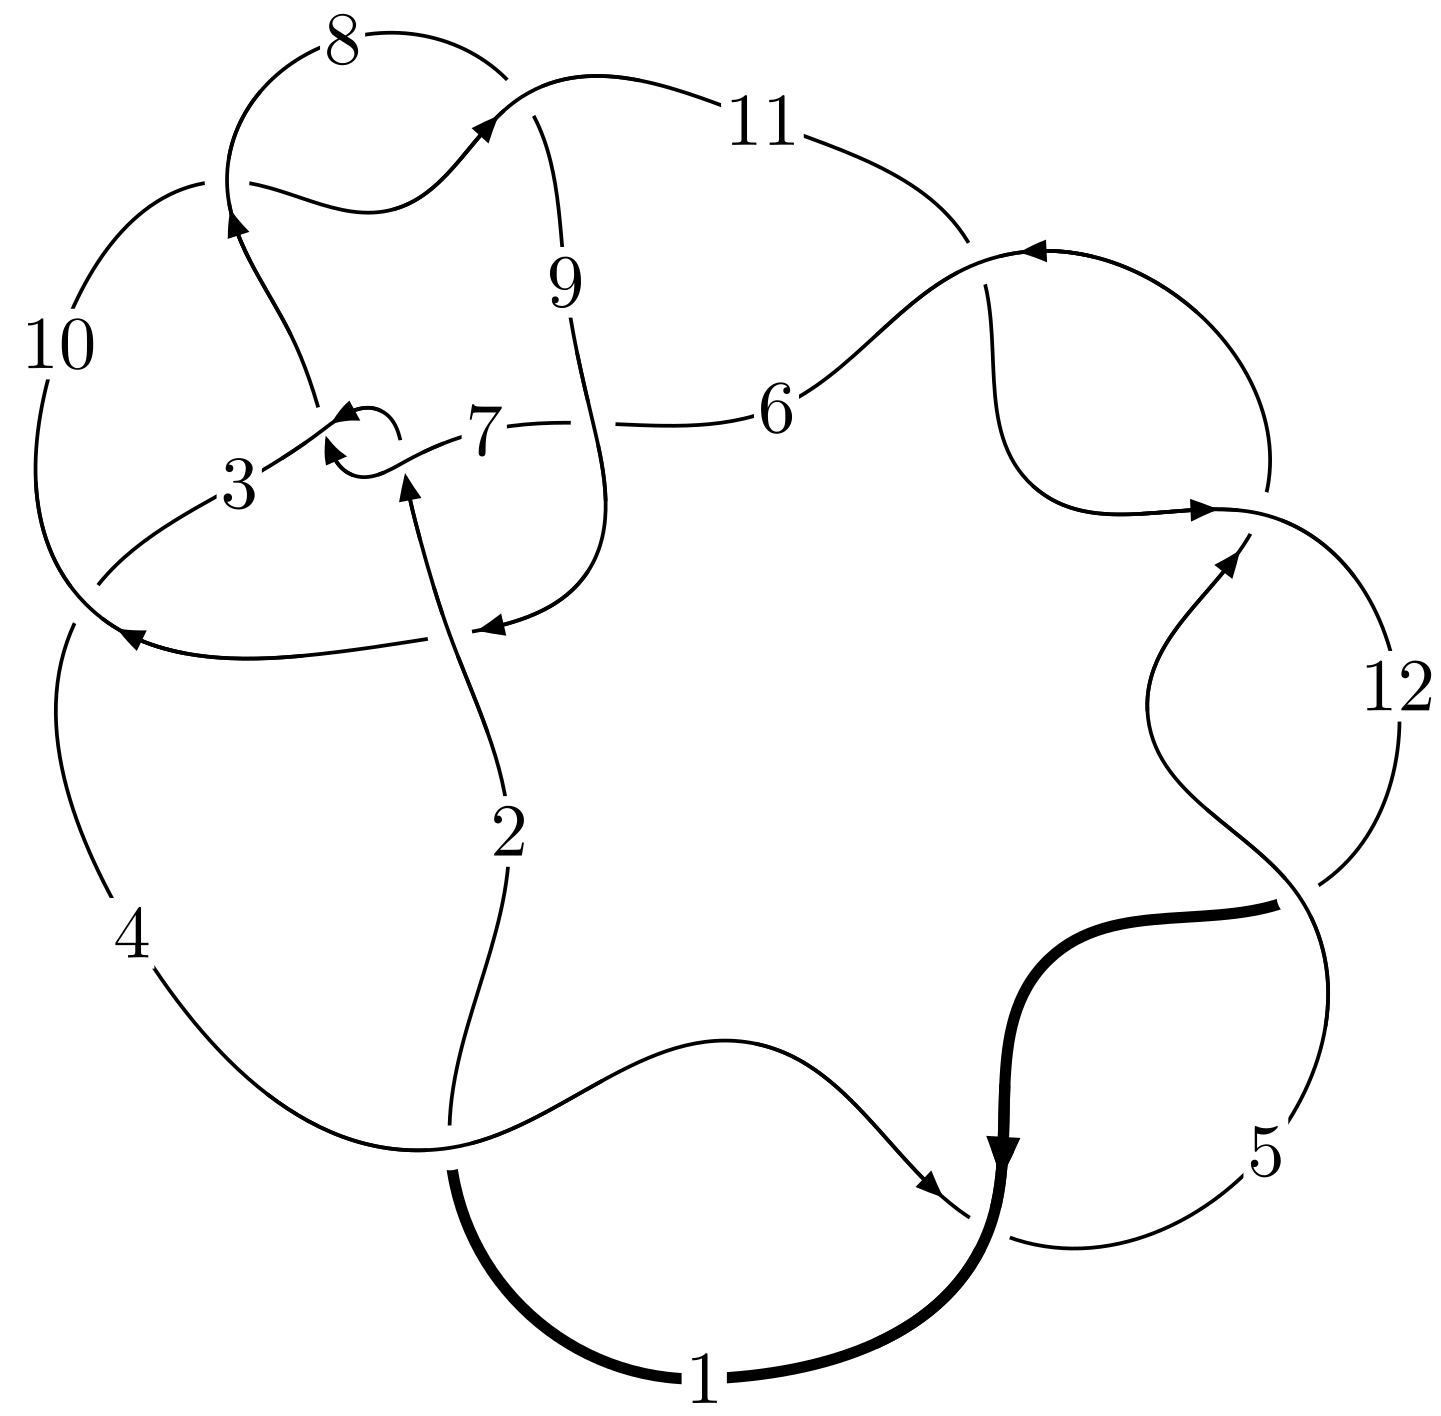
\includegraphics[width=112pt]{../../../GIT/diagram.site/Diagrams/png/1896_12a_1095.png}\\
\ \ \ A knot diagram\footnotemark}&
\allowdisplaybreaks
\textbf{Linearized knot diagam} \\
\cline{2-2}
 &
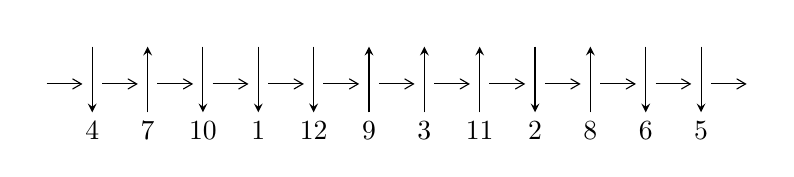
\begin{tikzpicture}[x=20pt, y=17pt]
	% nodes
	\node (C0) at (0, 0) {};
	\node (C1) at (1, 0) {};
	\node (C1U) at (1, +1) {};
	\node (C1D) at (1, -1) {4};

	\node (C2) at (2, 0) {};
	\node (C2U) at (2, +1) {};
	\node (C2D) at (2, -1) {7};

	\node (C3) at (3, 0) {};
	\node (C3U) at (3, +1) {};
	\node (C3D) at (3, -1) {10};

	\node (C4) at (4, 0) {};
	\node (C4U) at (4, +1) {};
	\node (C4D) at (4, -1) {1};

	\node (C5) at (5, 0) {};
	\node (C5U) at (5, +1) {};
	\node (C5D) at (5, -1) {12};

	\node (C6) at (6, 0) {};
	\node (C6U) at (6, +1) {};
	\node (C6D) at (6, -1) {9};

	\node (C7) at (7, 0) {};
	\node (C7U) at (7, +1) {};
	\node (C7D) at (7, -1) {3};

	\node (C8) at (8, 0) {};
	\node (C8U) at (8, +1) {};
	\node (C8D) at (8, -1) {11};

	\node (C9) at (9, 0) {};
	\node (C9U) at (9, +1) {};
	\node (C9D) at (9, -1) {2};

	\node (C10) at (10, 0) {};
	\node (C10U) at (10, +1) {};
	\node (C10D) at (10, -1) {8};

	\node (C11) at (11, 0) {};
	\node (C11U) at (11, +1) {};
	\node (C11D) at (11, -1) {6};

	\node (C12) at (12, 0) {};
	\node (C12U) at (12, +1) {};
	\node (C12D) at (12, -1) {5};
	\node (C13) at (13, 0) {};

	% arrows
	\draw[->,>={angle 60}]
	(C0) edge (C1) (C1) edge (C2) (C2) edge (C3) (C3) edge (C4) (C4) edge (C5) (C5) edge (C6) (C6) edge (C7) (C7) edge (C8) (C8) edge (C9) (C9) edge (C10) (C10) edge (C11) (C11) edge (C12) (C12) edge (C13) ;	\draw[->,>=stealth]
	(C1U) edge (C1D) (C2D) edge (C2U) (C3U) edge (C3D) (C4U) edge (C4D) (C5U) edge (C5D) (C6D) edge (C6U) (C7D) edge (C7U) (C8D) edge (C8U) (C9U) edge (C9D) (C10D) edge (C10U) (C11U) edge (C11D) (C12U) edge (C12D) ;
	\end{tikzpicture} \\
\hhline{~~} \\& 
\textbf{Solving Sequence} \\ \cline{2-2} 
 &
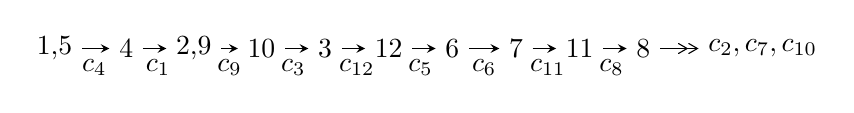
\begin{tikzpicture}[x=23pt, y=7pt]
	% node
	\node (A0) at (-1/8, 0) {1,5};
	\node (A1) at (1, 0) {4};
	\node (A2) at (33/16, 0) {2,9};
	\node (A3) at (25/8, 0) {10};
	\node (A4) at (33/8, 0) {3};
	\node (A5) at (41/8, 0) {12};
	\node (A6) at (49/8, 0) {6};
	\node (A7) at (57/8, 0) {7};
	\node (A8) at (65/8, 0) {11};
	\node (A9) at (73/8, 0) {8};
	\node (C1) at (1/2, -1) {$c_{4}$};
	\node (C2) at (3/2, -1) {$c_{1}$};
	\node (C3) at (21/8, -1) {$c_{9}$};
	\node (C4) at (29/8, -1) {$c_{3}$};
	\node (C5) at (37/8, -1) {$c_{12}$};
	\node (C6) at (45/8, -1) {$c_{5}$};
	\node (C7) at (53/8, -1) {$c_{6}$};
	\node (C8) at (61/8, -1) {$c_{11}$};
	\node (C9) at (69/8, -1) {$c_{8}$};
	\node (A10) at (11, 0) {$c_{2},c_{7},c_{10}$};

	% edge
	\draw[->,>=stealth]	
	(A0) edge (A1) (A1) edge (A2) (A2) edge (A3) (A3) edge (A4) (A4) edge (A5) (A5) edge (A6) (A6) edge (A7) (A7) edge (A8) (A8) edge (A9) ;
	\draw[->>,>={angle 60}]	
	(A9) edge (A10);
\end{tikzpicture} \\ 

\end{tabular} \\

\footnotetext{
The image of knot diagram is generated by the software ``\textbf{Draw programme}" developed by Andrew Bartholomew(\url{http://www.layer8.co.uk/maths/draw/index.htm\#Running-draw}), where we modified some parts for our purpose(\url{https://github.com/CATsTAILs/LinksPainter}).
}\phantom \\ \newline 
\centering \textbf{Ideals for irreducible components\footnotemark of $X_{\text{par}}$} 
 
\begin{align*}
I^u_{1}&=\langle 
1.34837\times10^{27} u^{52}-2.41782\times10^{27} u^{51}+\cdots+2.76539\times10^{27} b-4.01656\times10^{27},\\
\phantom{I^u_{1}}&\phantom{= \langle  }-3.41977\times10^{27} u^{52}+6.63330\times10^{27} u^{51}+\cdots+5.53078\times10^{27} a+3.25207\times10^{27},\;u^{53}-2 u^{52}+\cdots-3 u+1\rangle \\
I^u_{2}&=\langle 
u^3+2 u^2+4 b+5 u+3,\;-5 u^3-2 u^2+8 a-9 u-3,\;u^4+u^3+3 u^2+2 u+1\rangle \\
\\
\end{align*}
\raggedright * 2 irreducible components of $\dim_{\mathbb{C}}=0$, with total 57 representations.\\
\footnotetext{All coefficients of polynomials are rational numbers. But the coefficients are sometimes approximated in decimal forms when there is not enough margin.}
\newpage
\renewcommand{\arraystretch}{1}
\centering \section*{I. $I^u_{1}= \langle 1.35\times10^{27} u^{52}-2.42\times10^{27} u^{51}+\cdots+2.77\times10^{27} b-4.02\times10^{27},\;-3.42\times10^{27} u^{52}+6.63\times10^{27} u^{51}+\cdots+5.53\times10^{27} a+3.25\times10^{27},\;u^{53}-2 u^{52}+\cdots-3 u+1 \rangle$}
\flushleft \textbf{(i) Arc colorings}\\
\begin{tabular}{m{7pt} m{180pt} m{7pt} m{180pt} }
\flushright $a_{1}=$&$\begin{pmatrix}0\\u\end{pmatrix}$ \\
\flushright $a_{5}=$&$\begin{pmatrix}1\\0\end{pmatrix}$ \\
\flushright $a_{4}=$&$\begin{pmatrix}1\\- u^2\end{pmatrix}$ \\
\flushright $a_{2}=$&$\begin{pmatrix}- u\\u^3+u\end{pmatrix}$ \\
\flushright $a_{9}=$&$\begin{pmatrix}0.618315 u^{52}-1.19934 u^{51}+\cdots+8.80138 u-0.587995\\-0.487586 u^{52}+0.874316 u^{51}+\cdots-2.83559 u+1.45244\end{pmatrix}$ \\
\flushright $a_{10}=$&$\begin{pmatrix}0.530284 u^{52}-1.04842 u^{51}+\cdots+8.32484 u-0.480894\\-0.408912 u^{52}+0.748136 u^{51}+\cdots-2.37166 u+1.32020\end{pmatrix}$ \\
\flushright $a_{3}=$&$\begin{pmatrix}0.0838946 u^{52}-0.639715 u^{51}+\cdots-3.71956 u-0.610289\\-0.0738827 u^{52}+0.330937 u^{51}+\cdots+4.07454 u-0.785735\end{pmatrix}$ \\
\flushright $a_{12}=$&$\begin{pmatrix}u\\u\end{pmatrix}$ \\
\flushright $a_{6}=$&$\begin{pmatrix}u^2+1\\u^2\end{pmatrix}$ \\
\flushright $a_{7}=$&$\begin{pmatrix}-1.11189 u^{52}+2.28145 u^{51}+\cdots-7.30635 u-0.400627\\0.307946 u^{52}-0.571956 u^{51}+\cdots+6.37995 u-2.10022\end{pmatrix}$ \\
\flushright $a_{11}=$&$\begin{pmatrix}u^3+2 u\\u^3+u\end{pmatrix}$ \\
\flushright $a_{8}=$&$\begin{pmatrix}0.780510 u^{52}-1.54138 u^{51}+\cdots+7.33530 u-1.15081\\-0.419078 u^{52}+0.718479 u^{51}+\cdots-3.61371 u+1.17045\end{pmatrix}$\\&\end{tabular}
\flushleft \textbf{(ii) Obstruction class $= -1$}\\~\\
\flushleft \textbf{(iii) Cusp Shapes $= -0.212314 u^{52}+1.34571 u^{51}+\cdots+2.23825 u+7.42547$}\\~\\
\newpage\renewcommand{\arraystretch}{1}
\flushleft \textbf{(iv) u-Polynomials at the component}\newline \\
\begin{tabular}{m{50pt}|m{274pt}}
Crossings & \hspace{64pt}u-Polynomials at each crossing \\
\hline $$\begin{aligned}c_{1},c_{4},c_{5}\\c_{11},c_{12}\end{aligned}$$&$\begin{aligned}
&u^{53}-2 u^{52}+\cdots-3 u+1
\end{aligned}$\\
\hline $$\begin{aligned}c_{2},c_{7}\end{aligned}$$&$\begin{aligned}
&u^{53}+2 u^{52}+\cdots+3 u-1
\end{aligned}$\\
\hline $$\begin{aligned}c_{3}\end{aligned}$$&$\begin{aligned}
&8(8 u^{53}-11 u^{52}+\cdots+480 u+3943)
\end{aligned}$\\
\hline $$\begin{aligned}c_{6}\end{aligned}$$&$\begin{aligned}
&8(8 u^{53}-7 u^{52}+\cdots+348462 u+61297)
\end{aligned}$\\
\hline $$\begin{aligned}c_{8},c_{10}\end{aligned}$$&$\begin{aligned}
&u^{53}+5 u^{52}+\cdots-17 u-64
\end{aligned}$\\
\hline $$\begin{aligned}c_{9}\end{aligned}$$&$\begin{aligned}
&u^{53}-3 u^{52}+\cdots-576 u+1024
\end{aligned}$\\
\hline
\end{tabular}\\~\\
\newpage\renewcommand{\arraystretch}{1}
\flushleft \textbf{(v) Riley Polynomials at the component}\newline \\
\begin{tabular}{m{50pt}|m{274pt}}
Crossings & \hspace{64pt}Riley Polynomials at each crossing \\
\hline $$\begin{aligned}c_{1},c_{4},c_{5}\\c_{11},c_{12}\end{aligned}$$&$\begin{aligned}
&y^{53}+72 y^{52}+\cdots-13 y-1
\end{aligned}$\\
\hline $$\begin{aligned}c_{2},c_{7}\end{aligned}$$&$\begin{aligned}
&y^{53}-36 y^{52}+\cdots-13 y-1
\end{aligned}$\\
\hline $$\begin{aligned}c_{3}\end{aligned}$$&$\begin{aligned}
&64(64 y^{53}+2007 y^{52}+\cdots-9.98193\times10^{7} y-1.55472\times10^{7})
\end{aligned}$\\
\hline $$\begin{aligned}c_{6}\end{aligned}$$&$\begin{aligned}
&64(64 y^{53}-3105 y^{52}+\cdots+2.44146\times10^{10} y-3.75732\times10^{9})
\end{aligned}$\\
\hline $$\begin{aligned}c_{8},c_{10}\end{aligned}$$&$\begin{aligned}
&y^{53}-49 y^{52}+\cdots+68129 y-4096
\end{aligned}$\\
\hline $$\begin{aligned}c_{9}\end{aligned}$$&$\begin{aligned}
&y^{53}+27 y^{52}+\cdots-8925184 y-1048576
\end{aligned}$\\
\hline
\end{tabular}\\~\\
\newpage\flushleft \textbf{(vi) Complex Volumes and Cusp Shapes}
$$\begin{array}{c|c|c}  
\text{Solutions to }I^u_{1}& \I (\text{vol} + \sqrt{-1}CS) & \text{Cusp shape}\\
 \hline 
\begin{aligned}
u &= \phantom{-}0.097309 + 1.013130 I \\
a &= \phantom{-}1.06909 + 1.45901 I \\
b &= -0.293233 - 0.247581 I\end{aligned}
 & \phantom{-}5.81488 + 0.01278 I & \phantom{-0.000000 } 0 \\ \hline\begin{aligned}
u &= \phantom{-}0.097309 - 1.013130 I \\
a &= \phantom{-}1.06909 - 1.45901 I \\
b &= -0.293233 + 0.247581 I\end{aligned}
 & \phantom{-}5.81488 - 0.01278 I & \phantom{-0.000000 } 0 \\ \hline\begin{aligned}
u &= -0.170586 + 1.030690 I \\
a &= -0.621933 + 0.377743 I \\
b &= \phantom{-}0.745819 + 0.222778 I\end{aligned}
 & \phantom{-}2.87981 + 2.52887 I & \phantom{-0.000000 } 0 \\ \hline\begin{aligned}
u &= -0.170586 - 1.030690 I \\
a &= -0.621933 - 0.377743 I \\
b &= \phantom{-}0.745819 - 0.222778 I\end{aligned}
 & \phantom{-}2.87981 - 2.52887 I & \phantom{-0.000000 } 0 \\ \hline\begin{aligned}
u &= \phantom{-}0.043294 + 1.080920 I \\
a &= \phantom{-}0.98039 - 1.04863 I \\
b &= -0.415517 - 0.941732 I\end{aligned}
 & \phantom{-}5.95677 - 1.10474 I & \phantom{-0.000000 } 0 \\ \hline\begin{aligned}
u &= \phantom{-}0.043294 - 1.080920 I \\
a &= \phantom{-}0.98039 + 1.04863 I \\
b &= -0.415517 + 0.941732 I\end{aligned}
 & \phantom{-}5.95677 + 1.10474 I & \phantom{-0.000000 } 0 \\ \hline\begin{aligned}
u &= \phantom{-}0.183709 + 1.096700 I \\
a &= \phantom{-}0.615073 + 0.266917 I \\
b &= -1.40828 + 0.31772 I\end{aligned}
 & \phantom{-}6.45837 - 5.82425 I & \phantom{-0.000000 } 0 \\ \hline\begin{aligned}
u &= \phantom{-}0.183709 - 1.096700 I \\
a &= \phantom{-}0.615073 - 0.266917 I \\
b &= -1.40828 - 0.31772 I\end{aligned}
 & \phantom{-}6.45837 + 5.82425 I & \phantom{-0.000000 } 0 \\ \hline\begin{aligned}
u &= -0.060804 + 1.151400 I \\
a &= -0.235310 - 0.453905 I \\
b &= \phantom{-}1.07199 - 1.72723 I\end{aligned}
 & \phantom{-}10.49640 + 2.30207 I & \phantom{-0.000000 } 0 \\ \hline\begin{aligned}
u &= -0.060804 - 1.151400 I \\
a &= -0.235310 + 0.453905 I \\
b &= \phantom{-}1.07199 + 1.72723 I\end{aligned}
 & \phantom{-}10.49640 - 2.30207 I & \phantom{-0.000000 } 0\\
 \hline 
 \end{array}$$\newpage$$\begin{array}{c|c|c}  
\text{Solutions to }I^u_{1}& \I (\text{vol} + \sqrt{-1}CS) & \text{Cusp shape}\\
 \hline 
\begin{aligned}
u &= -0.697220 + 0.415437 I \\
a &= \phantom{-}0.367510 - 0.569917 I \\
b &= \phantom{-}0.598266 + 0.118968 I\end{aligned}
 & \phantom{-}2.58042 + 2.27566 I & \phantom{-}5.54808 - 4.42595 I \\ \hline\begin{aligned}
u &= -0.697220 - 0.415437 I \\
a &= \phantom{-}0.367510 + 0.569917 I \\
b &= \phantom{-}0.598266 - 0.118968 I\end{aligned}
 & \phantom{-}2.58042 - 2.27566 I & \phantom{-}5.54808 + 4.42595 I \\ \hline\begin{aligned}
u &= \phantom{-}0.348979 + 1.163470 I \\
a &= -0.789223 - 0.400014 I \\
b &= \phantom{-}0.803943 + 0.133985 I\end{aligned}
 & \phantom{-}12.4109 - 11.7818 I & \phantom{-0.000000 } 0 \\ \hline\begin{aligned}
u &= \phantom{-}0.348979 - 1.163470 I \\
a &= -0.789223 + 0.400014 I \\
b &= \phantom{-}0.803943 - 0.133985 I\end{aligned}
 & \phantom{-}12.4109 + 11.7818 I & \phantom{-0.000000 } 0 \\ \hline\begin{aligned}
u &= \phantom{-}0.400033 + 1.148970 I \\
a &= -0.209336 - 0.368266 I \\
b &= \phantom{-}0.537132 + 0.552257 I\end{aligned}
 & \phantom{-}11.91410 + 0.46291 I & \phantom{-0.000000 } 0 \\ \hline\begin{aligned}
u &= \phantom{-}0.400033 - 1.148970 I \\
a &= -0.209336 + 0.368266 I \\
b &= \phantom{-}0.537132 - 0.552257 I\end{aligned}
 & \phantom{-}11.91410 - 0.46291 I & \phantom{-0.000000 } 0 \\ \hline\begin{aligned}
u &= \phantom{-}0.638183 + 0.414259 I \\
a &= -0.885666 - 0.562368 I \\
b &= -0.877415 + 0.319431 I\end{aligned}
 & \phantom{-}7.44710 - 8.39986 I & \phantom{-}4.21700 + 7.17865 I \\ \hline\begin{aligned}
u &= \phantom{-}0.638183 - 0.414259 I \\
a &= -0.885666 + 0.562368 I \\
b &= -0.877415 - 0.319431 I\end{aligned}
 & \phantom{-}7.44710 + 8.39986 I & \phantom{-}4.21700 - 7.17865 I \\ \hline\begin{aligned}
u &= \phantom{-}0.673423 + 0.351163 I \\
a &= -0.043002 - 1.043460 I \\
b &= -0.615958 - 0.222480 I\end{aligned}
 & \phantom{-}7.23787 + 4.15053 I & \phantom{-}4.88455 - 1.78073 I \\ \hline\begin{aligned}
u &= \phantom{-}0.673423 - 0.351163 I \\
a &= -0.043002 + 1.043460 I \\
b &= -0.615958 + 0.222480 I\end{aligned}
 & \phantom{-}7.23787 - 4.15053 I & \phantom{-}4.88455 + 1.78073 I\\
 \hline 
 \end{array}$$\newpage$$\begin{array}{c|c|c}  
\text{Solutions to }I^u_{1}& \I (\text{vol} + \sqrt{-1}CS) & \text{Cusp shape}\\
 \hline 
\begin{aligned}
u &= -0.369763 + 1.185950 I \\
a &= \phantom{-}0.519790 - 0.236280 I \\
b &= -0.595932 + 0.252414 I\end{aligned}
 & \phantom{-}7.64201 + 5.93448 I & \phantom{-0.000000 } 0 \\ \hline\begin{aligned}
u &= -0.369763 - 1.185950 I \\
a &= \phantom{-}0.519790 + 0.236280 I \\
b &= -0.595932 - 0.252414 I\end{aligned}
 & \phantom{-}7.64201 - 5.93448 I & \phantom{-0.000000 } 0 \\ \hline\begin{aligned}
u &= -0.284491 + 0.620702 I \\
a &= \phantom{-}0.089749 + 0.451278 I \\
b &= \phantom{-}0.078976 + 0.540092 I\end{aligned}
 & \phantom{-}0.33460 + 1.76623 I & -3.26918 - 5.78660 I \\ \hline\begin{aligned}
u &= -0.284491 - 0.620702 I \\
a &= \phantom{-}0.089749 - 0.451278 I \\
b &= \phantom{-}0.078976 - 0.540092 I\end{aligned}
 & \phantom{-}0.33460 - 1.76623 I & -3.26918 + 5.78660 I \\ \hline\begin{aligned}
u &= \phantom{-}0.392790 + 0.323030 I \\
a &= \phantom{-}2.01412 + 0.72401 I \\
b &= \phantom{-}0.535471 - 0.302352 I\end{aligned}
 & \phantom{-}1.98439 - 3.87908 I & \phantom{-}1.02310 + 8.63789 I \\ \hline\begin{aligned}
u &= \phantom{-}0.392790 - 0.323030 I \\
a &= \phantom{-}2.01412 - 0.72401 I \\
b &= \phantom{-}0.535471 + 0.302352 I\end{aligned}
 & \phantom{-}1.98439 + 3.87908 I & \phantom{-}1.02310 - 8.63789 I \\ \hline\begin{aligned}
u &= -0.166207 + 0.454728 I \\
a &= -1.06595 + 3.13668 I \\
b &= -0.335420 - 0.115389 I\end{aligned}
 & \phantom{-}5.39007 + 1.57476 I & \phantom{-}8.26638 - 4.56003 I \\ \hline\begin{aligned}
u &= -0.166207 - 0.454728 I \\
a &= -1.06595 - 3.13668 I \\
b &= -0.335420 + 0.115389 I\end{aligned}
 & \phantom{-}5.39007 - 1.57476 I & \phantom{-}8.26638 + 4.56003 I \\ \hline\begin{aligned}
u &= -0.400179 + 0.184061 I \\
a &= -1.113230 + 0.254594 I \\
b &= -0.294175 - 0.144169 I\end{aligned}
 & -0.906294 + 0.638936 I & -7.84585 - 3.54441 I \\ \hline\begin{aligned}
u &= -0.400179 - 0.184061 I \\
a &= -1.113230 - 0.254594 I \\
b &= -0.294175 + 0.144169 I\end{aligned}
 & -0.906294 - 0.638936 I & -7.84585 + 3.54441 I\\
 \hline 
 \end{array}$$\newpage$$\begin{array}{c|c|c}  
\text{Solutions to }I^u_{1}& \I (\text{vol} + \sqrt{-1}CS) & \text{Cusp shape}\\
 \hline 
\begin{aligned}
u &= \phantom{-}0.337976 + 0.277219 I \\
a &= \phantom{-}0.080619 + 1.061220 I \\
b &= \phantom{-}0.612117 + 0.741472 I\end{aligned}
 & \phantom{-}1.91837 + 1.38671 I & \phantom{-}0.37102 + 1.92125 I \\ \hline\begin{aligned}
u &= \phantom{-}0.337976 - 0.277219 I \\
a &= \phantom{-}0.080619 - 1.061220 I \\
b &= \phantom{-}0.612117 - 0.741472 I\end{aligned}
 & \phantom{-}1.91837 - 1.38671 I & \phantom{-}0.37102 - 1.92125 I \\ \hline\begin{aligned}
u &= -0.08231 + 1.59104 I \\
a &= \phantom{-}0.098365 + 0.362333 I \\
b &= \phantom{-}0.061723 + 0.202369 I\end{aligned}
 & \phantom{-}7.93934 + 3.04380 I & \phantom{-0.000000 } 0 \\ \hline\begin{aligned}
u &= -0.08231 - 1.59104 I \\
a &= \phantom{-}0.098365 - 0.362333 I \\
b &= \phantom{-}0.061723 - 0.202369 I\end{aligned}
 & \phantom{-}7.93934 - 3.04380 I & \phantom{-0.000000 } 0 \\ \hline\begin{aligned}
u &= -0.309511\phantom{ +0.000000I} \\
a &= -0.285999\phantom{ +0.000000I} \\
b &= -1.99031\phantom{ +0.000000I}\end{aligned}
 & \phantom{-}3.96788\phantom{ +0.000000I} & -11.2160\phantom{ +0.000000I} \\ \hline\begin{aligned}
u &= \phantom{-}0.146397 + 0.259785 I \\
a &= \phantom{-}0.26789 + 2.10948 I \\
b &= \phantom{-}0.661555 - 0.546534 I\end{aligned}
 & \phantom{-}1.70235 - 0.53525 I & \phantom{-}5.77546 - 2.21892 I \\ \hline\begin{aligned}
u &= \phantom{-}0.146397 - 0.259785 I \\
a &= \phantom{-}0.26789 - 2.10948 I \\
b &= \phantom{-}0.661555 + 0.546534 I\end{aligned}
 & \phantom{-}1.70235 + 0.53525 I & \phantom{-}5.77546 + 2.21892 I \\ \hline\begin{aligned}
u &= \phantom{-}0.02066 + 1.73571 I \\
a &= -2.64807 - 1.49652 I \\
b &= -5.03892 - 2.83332 I\end{aligned}
 & \phantom{-}15.7407 - 0.4328 I & \phantom{-0.000000 } 0 \\ \hline\begin{aligned}
u &= \phantom{-}0.02066 - 1.73571 I \\
a &= -2.64807 + 1.49652 I \\
b &= -5.03892 + 2.83332 I\end{aligned}
 & \phantom{-}15.7407 + 0.4328 I & \phantom{-0.000000 } 0 \\ \hline\begin{aligned}
u &= -0.03957 + 1.74066 I \\
a &= \phantom{-}2.21887 - 0.02192 I \\
b &= \phantom{-}3.84932 - 0.12795 I\end{aligned}
 & \phantom{-}12.88280 + 3.36516 I & \phantom{-0.000000 } 0\\
 \hline 
 \end{array}$$\newpage$$\begin{array}{c|c|c}  
\text{Solutions to }I^u_{1}& \I (\text{vol} + \sqrt{-1}CS) & \text{Cusp shape}\\
 \hline 
\begin{aligned}
u &= -0.03957 - 1.74066 I \\
a &= \phantom{-}2.21887 + 0.02192 I \\
b &= \phantom{-}3.84932 + 0.12795 I\end{aligned}
 & \phantom{-}12.88280 - 3.36516 I & \phantom{-0.000000 } 0 \\ \hline\begin{aligned}
u &= \phantom{-}0.00922 + 1.75210 I \\
a &= -1.76414 + 0.35710 I \\
b &= -3.28376 + 1.33114 I\end{aligned}
 & \phantom{-}16.2367 - 1.3130 I & \phantom{-0.000000 } 0 \\ \hline\begin{aligned}
u &= \phantom{-}0.00922 - 1.75210 I \\
a &= -1.76414 - 0.35710 I \\
b &= -3.28376 - 1.33114 I\end{aligned}
 & \phantom{-}16.2367 + 1.3130 I & \phantom{-0.000000 } 0 \\ \hline\begin{aligned}
u &= \phantom{-}0.04422 + 1.75495 I \\
a &= -2.98121 + 0.32099 I \\
b &= -4.98803 + 0.54697 I\end{aligned}
 & \phantom{-}16.7715 - 6.7678 I & \phantom{-0.000000 } 0 \\ \hline\begin{aligned}
u &= \phantom{-}0.04422 - 1.75495 I \\
a &= -2.98121 - 0.32099 I \\
b &= -4.98803 - 0.54697 I\end{aligned}
 & \phantom{-}16.7715 + 6.7678 I & \phantom{-0.000000 } 0 \\ \hline\begin{aligned}
u &= -0.01406 + 1.76783 I \\
a &= \phantom{-}1.92068 - 1.63644 I \\
b &= \phantom{-}3.22687 - 2.19591 I\end{aligned}
 & -18.3521 + 2.6162 I & \phantom{-0.000000 } 0 \\ \hline\begin{aligned}
u &= -0.01406 - 1.76783 I \\
a &= \phantom{-}1.92068 + 1.63644 I \\
b &= \phantom{-}3.22687 + 2.19591 I\end{aligned}
 & -18.3521 - 2.6162 I & \phantom{-0.000000 } 0 \\ \hline\begin{aligned}
u &= \phantom{-}0.09238 + 1.77000 I \\
a &= \phantom{-}2.54868 + 0.19679 I \\
b &= \phantom{-}4.60054 + 0.16183 I\end{aligned}
 & -16.5345 - 13.6959 I & \phantom{-0.000000 } 0 \\ \hline\begin{aligned}
u &= \phantom{-}0.09238 - 1.77000 I \\
a &= \phantom{-}2.54868 - 0.19679 I \\
b &= \phantom{-}4.60054 - 0.16183 I\end{aligned}
 & -16.5345 + 13.6959 I & \phantom{-0.000000 } 0 \\ \hline\begin{aligned}
u &= \phantom{-}0.10675 + 1.77331 I \\
a &= \phantom{-}1.50063 + 0.72497 I \\
b &= \phantom{-}2.72216 + 1.03571 I\end{aligned}
 & -17.0899 - 1.7379 I & \phantom{-0.000000 } 0\\
 \hline 
 \end{array}$$\newpage$$\begin{array}{c|c|c}  
\text{Solutions to }I^u_{1}& \I (\text{vol} + \sqrt{-1}CS) & \text{Cusp shape}\\
 \hline 
\begin{aligned}
u &= \phantom{-}0.10675 - 1.77331 I \\
a &= \phantom{-}1.50063 - 0.72497 I \\
b &= \phantom{-}2.72216 - 1.03571 I\end{aligned}
 & -17.0899 + 1.7379 I & \phantom{-0.000000 } 0 \\ \hline\begin{aligned}
u &= -0.09538 + 1.77635 I \\
a &= -1.97891 + 0.19640 I \\
b &= -3.58909 + 0.12592 I\end{aligned}
 & \phantom{-}18.2869 + 7.9543 I & \phantom{-0.000000 } 0 \\ \hline\begin{aligned}
u &= -0.09538 - 1.77635 I \\
a &= -1.97891 - 0.19640 I \\
b &= -3.58909 - 0.12592 I\end{aligned}
 & \phantom{-}18.2869 - 7.9543 I & \phantom{-0.000000 } 0\\
 \hline 
 \end{array}$$\newpage\newpage\renewcommand{\arraystretch}{1}
\centering \section*{II. $I^u_{2}= \langle u^3+2 u^2+4 b+5 u+3,\;-5 u^3-2 u^2+8 a-9 u-3,\;u^4+u^3+3 u^2+2 u+1 \rangle$}
\flushleft \textbf{(i) Arc colorings}\\
\begin{tabular}{m{7pt} m{180pt} m{7pt} m{180pt} }
\flushright $a_{1}=$&$\begin{pmatrix}0\\u\end{pmatrix}$ \\
\flushright $a_{5}=$&$\begin{pmatrix}1\\0\end{pmatrix}$ \\
\flushright $a_{4}=$&$\begin{pmatrix}1\\- u^2\end{pmatrix}$ \\
\flushright $a_{2}=$&$\begin{pmatrix}- u\\u^3+u\end{pmatrix}$ \\
\flushright $a_{9}=$&$\begin{pmatrix}\frac{5}{8} u^3+\frac{1}{4} u^2+\frac{9}{8} u+\frac{3}{8}\\-\frac{1}{4} u^3-\frac{1}{2} u^2-\frac{5}{4} u-\frac{3}{4}\end{pmatrix}$ \\
\flushright $a_{10}=$&$\begin{pmatrix}\frac{5}{8} u^3+\frac{1}{4} u^2+\frac{9}{8} u+\frac{3}{8}\\-\frac{1}{4} u^3-\frac{1}{2} u^2-\frac{5}{4} u-\frac{3}{4}\end{pmatrix}$ \\
\flushright $a_{3}=$&$\begin{pmatrix}0.109375 u^{3}+0.0937500 u^{2}+0.171875 u+0.765625\\0.0312500 u^{3}-0.687500 u^{2}-0.0937500 u+0.218750\end{pmatrix}$ \\
\flushright $a_{12}=$&$\begin{pmatrix}u\\u\end{pmatrix}$ \\
\flushright $a_{6}=$&$\begin{pmatrix}u^2+1\\u^2\end{pmatrix}$ \\
\flushright $a_{7}=$&$\begin{pmatrix}0.296875 u^{3}+0.968750 u^{2}+0.609375 u+1.07813\\-0.343750 u^{3}+0.562500 u^{2}-0.968750 u-0.406250\end{pmatrix}$ \\
\flushright $a_{11}=$&$\begin{pmatrix}u^3+2 u\\u^3+u\end{pmatrix}$ \\
\flushright $a_{8}=$&$\begin{pmatrix}-\frac{3}{8} u^3+\frac{1}{4} u^2-\frac{7}{8} u+\frac{3}{8}\\-\frac{5}{4} u^3-\frac{1}{2} u^2-\frac{9}{4} u-\frac{3}{4}\end{pmatrix}$\\&\end{tabular}
\flushleft \textbf{(ii) Obstruction class $= 1$}\\~\\
\flushleft \textbf{(iii) Cusp Shapes $= -\frac{233}{64} u^3-\frac{205}{32} u^2-\frac{805}{64} u-\frac{159}{64}$}\\~\\
\newpage\renewcommand{\arraystretch}{1}
\flushleft \textbf{(iv) u-Polynomials at the component}\newline \\
\begin{tabular}{m{50pt}|m{274pt}}
Crossings & \hspace{64pt}u-Polynomials at each crossing \\
\hline $$\begin{aligned}c_{1},c_{11},c_{12}\end{aligned}$$&$\begin{aligned}
&u^4- u^3+3 u^2-2 u+1
\end{aligned}$\\
\hline $$\begin{aligned}c_{2}\end{aligned}$$&$\begin{aligned}
&u^4- u^3+u^2+1
\end{aligned}$\\
\hline $$\begin{aligned}c_{3}\end{aligned}$$&$\begin{aligned}
&8(8 u^4+3 u^3+6 u^2+u+1)
\end{aligned}$\\
\hline $$\begin{aligned}c_{4},c_{5}\end{aligned}$$&$\begin{aligned}
&u^4+u^3+3 u^2+2 u+1
\end{aligned}$\\
\hline $$\begin{aligned}c_{6}\end{aligned}$$&$\begin{aligned}
&8(8 u^4+15 u^3+12 u^2+5 u+1)
\end{aligned}$\\
\hline $$\begin{aligned}c_{7}\end{aligned}$$&$\begin{aligned}
&u^4+u^3+u^2+1
\end{aligned}$\\
\hline $$\begin{aligned}c_{8}\end{aligned}$$&$\begin{aligned}
&(u+1)^4
\end{aligned}$\\
\hline $$\begin{aligned}c_{9}\end{aligned}$$&$\begin{aligned}
&u^4
\end{aligned}$\\
\hline $$\begin{aligned}c_{10}\end{aligned}$$&$\begin{aligned}
&(u-1)^4
\end{aligned}$\\
\hline
\end{tabular}\\~\\
\newpage\renewcommand{\arraystretch}{1}
\flushleft \textbf{(v) Riley Polynomials at the component}\newline \\
\begin{tabular}{m{50pt}|m{274pt}}
Crossings & \hspace{64pt}Riley Polynomials at each crossing \\
\hline $$\begin{aligned}c_{1},c_{4},c_{5}\\c_{11},c_{12}\end{aligned}$$&$\begin{aligned}
&y^4+5 y^3+7 y^2+2 y+1
\end{aligned}$\\
\hline $$\begin{aligned}c_{2},c_{7}\end{aligned}$$&$\begin{aligned}
&y^4+y^3+3 y^2+2 y+1
\end{aligned}$\\
\hline $$\begin{aligned}c_{3}\end{aligned}$$&$\begin{aligned}
&64(64 y^4+87 y^3+46 y^2+11 y+1)
\end{aligned}$\\
\hline $$\begin{aligned}c_{6}\end{aligned}$$&$\begin{aligned}
&64(64 y^4-33 y^3+10 y^2- y+1)
\end{aligned}$\\
\hline $$\begin{aligned}c_{8},c_{10}\end{aligned}$$&$\begin{aligned}
&(y-1)^4
\end{aligned}$\\
\hline $$\begin{aligned}c_{9}\end{aligned}$$&$\begin{aligned}
&y^4
\end{aligned}$\\
\hline
\end{tabular}\\~\\
\newpage\flushleft \textbf{(vi) Complex Volumes and Cusp Shapes}
$$\begin{array}{c|c|c}  
\text{Solutions to }I^u_{2}& \I (\text{vol} + \sqrt{-1}CS) & \text{Cusp shape}\\
 \hline 
\begin{aligned}
u &= -0.395123 + 0.506844 I \\
a &= \phantom{-}0.057058 + 0.537058 I \\
b &= -0.266417 - 0.460085 I\end{aligned}
 & \phantom{-}1.43393 + 1.41510 I & \phantom{-}2.24706 - 4.19946 I \\ \hline\begin{aligned}
u &= -0.395123 - 0.506844 I \\
a &= \phantom{-}0.057058 - 0.537058 I \\
b &= -0.266417 + 0.460085 I\end{aligned}
 & \phantom{-}1.43393 - 1.41510 I & \phantom{-}2.24706 + 4.19946 I \\ \hline\begin{aligned}
u &= -0.10488 + 1.55249 I \\
a &= \phantom{-}0.130442 - 0.641504 I \\
b &= \phantom{-}0.391417 - 0.855136 I\end{aligned}
 & \phantom{-}8.43568 + 3.16396 I & \phantom{-}11.44826 - 4.00508 I \\ \hline\begin{aligned}
u &= -0.10488 - 1.55249 I \\
a &= \phantom{-}0.130442 + 0.641504 I \\
b &= \phantom{-}0.391417 + 0.855136 I\end{aligned}
 & \phantom{-}8.43568 - 3.16396 I & \phantom{-}11.44826 + 4.00508 I\\
 \hline 
 \end{array}$$\newpage
\newpage\renewcommand{\arraystretch}{1}
\centering \section*{ III. u-Polynomials}
\begin{tabular}{m{50pt}|m{274pt}}
Crossings & \hspace{64pt}u-Polynomials at each crossing \\
\hline $$\begin{aligned}c_{1},c_{11},c_{12}\end{aligned}$$&$\begin{aligned}
&(u^4- u^3+3 u^2-2 u+1)(u^{53}-2 u^{52}+\cdots-3 u+1)
\end{aligned}$\\
\hline $$\begin{aligned}c_{2}\end{aligned}$$&$\begin{aligned}
&(u^4- u^3+u^2+1)(u^{53}+2 u^{52}+\cdots+3 u-1)
\end{aligned}$\\
\hline $$\begin{aligned}c_{3}\end{aligned}$$&$\begin{aligned}
&64(8 u^4+3 u^3+\cdots+u+1)(8 u^{53}-11 u^{52}+\cdots+480 u+3943)
\end{aligned}$\\
\hline $$\begin{aligned}c_{4},c_{5}\end{aligned}$$&$\begin{aligned}
&(u^4+u^3+3 u^2+2 u+1)(u^{53}-2 u^{52}+\cdots-3 u+1)
\end{aligned}$\\
\hline $$\begin{aligned}c_{6}\end{aligned}$$&$\begin{aligned}
&64(8 u^4+15 u^3+12 u^2+5 u+1)\\
&\cdot(8 u^{53}-7 u^{52}+\cdots+348462 u+61297)
\end{aligned}$\\
\hline $$\begin{aligned}c_{7}\end{aligned}$$&$\begin{aligned}
&(u^4+u^3+u^2+1)(u^{53}+2 u^{52}+\cdots+3 u-1)
\end{aligned}$\\
\hline $$\begin{aligned}c_{8}\end{aligned}$$&$\begin{aligned}
&((u+1)^4)(u^{53}+5 u^{52}+\cdots-17 u-64)
\end{aligned}$\\
\hline $$\begin{aligned}c_{9}\end{aligned}$$&$\begin{aligned}
&u^4(u^{53}-3 u^{52}+\cdots-576 u+1024)
\end{aligned}$\\
\hline $$\begin{aligned}c_{10}\end{aligned}$$&$\begin{aligned}
&((u-1)^4)(u^{53}+5 u^{52}+\cdots-17 u-64)
\end{aligned}$\\
\hline
\end{tabular}\newpage\renewcommand{\arraystretch}{1}
\centering \section*{ IV. Riley Polynomials}
\begin{tabular}{m{50pt}|m{274pt}}
Crossings & \hspace{64pt}Riley Polynomials at each crossing \\
\hline $$\begin{aligned}c_{1},c_{4},c_{5}\\c_{11},c_{12}\end{aligned}$$&$\begin{aligned}
&(y^4+5 y^3+7 y^2+2 y+1)(y^{53}+72 y^{52}+\cdots-13 y-1)
\end{aligned}$\\
\hline $$\begin{aligned}c_{2},c_{7}\end{aligned}$$&$\begin{aligned}
&(y^4+y^3+3 y^2+2 y+1)(y^{53}-36 y^{52}+\cdots-13 y-1)
\end{aligned}$\\
\hline $$\begin{aligned}c_{3}\end{aligned}$$&$\begin{aligned}
&4096(64 y^4+87 y^3+46 y^2+11 y+1)\\
&\cdot(64 y^{53}+2007 y^{52}+\cdots-99819282 y-15547249)
\end{aligned}$\\
\hline $$\begin{aligned}c_{6}\end{aligned}$$&$\begin{aligned}
&4096(64 y^4-33 y^3+10 y^2- y+1)\\
&\cdot(64 y^{53}-3105 y^{52}+\cdots+24414558770 y-3757322209)
\end{aligned}$\\
\hline $$\begin{aligned}c_{8},c_{10}\end{aligned}$$&$\begin{aligned}
&((y-1)^4)(y^{53}-49 y^{52}+\cdots+68129 y-4096)
\end{aligned}$\\
\hline $$\begin{aligned}c_{9}\end{aligned}$$&$\begin{aligned}
&y^4(y^{53}+27 y^{52}+\cdots-8925184 y-1048576)
\end{aligned}$\\
\hline
\end{tabular}
\vskip 2pc
\end{document}